

\subsubsection{Caso d'uso UCD0: Scenario principale}
\begin{center}
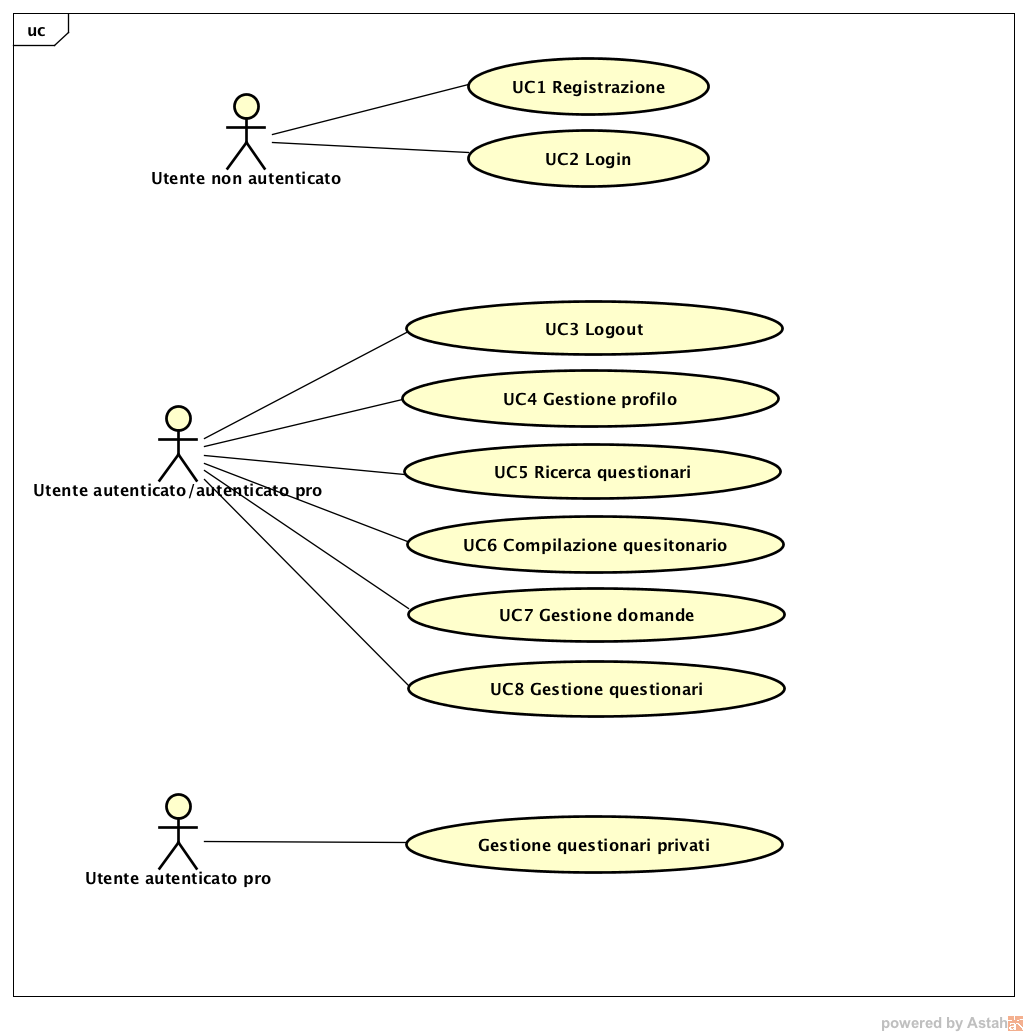
\includegraphics[scale=0.5]{/Users/Alberto/GitHub/Documenti/RR/AnalisiDeiRequisiti/sezioni/CasiD'uso/CasiD'usoDesktop/uc0.png}
\end{center}
\begin{itemize}
\item\textbf{Attori Principali}: Utente, Utente autenticato, Utente autenticato pro;
\item\textbf{Descrizione}: nella schermata principale proposta, l'utente può autenticarsi tramite l'apposto form di login oppure registrarsi nel sistema. Può inoltre recuperare la propria password. Infine un utente non autenticato può ricercare e compilare questionari \textit{pubblici} esistenti.\\
L'utente autenticato può, oltre a svolgere tutte le operazioni dell'utente non autenticato, eseguire il logout dal sistema e:
\begin{itemize}
\item Gestire le domande: può quindi inserire nuove domande nel sistema;
\item Gestire i questionari: può quindi creare questionari \textit{pubblici} oppure eliminare un questionario da lui creato;
\item Gestire il proprio profilo: può quindi modificare il proprio nome, cognome, indirizzo mail o password. Può visualizzare i questionari realizzati, compilari e le relative valutazioni ricevute.
\end{itemize}
L'utente autenticato \textbf{pro} può, oltre a svolgere tutte le operazioni dell'utente autenticato, gestire questionari \textit{privati}. Può quindi creare, modificare e proporre questionari \textit{privati} ad un numero limitato di utenti;
\item\textbf{Pre-condizione}: Il sistema è avviato e mostra la pagina iniziale dell'applicazione;
\item\textbf{Post-condizione}: Il sistema ha ricevuto tutte le informazioni dall'utente sulle operazioni che vuole eseguire.
\item\textbf{Scenario principale}:
\begin{itemize}
\item L'utente può registrarsi all'applicazione (UC1);
\item L'utente può eseguire il login all'applicazione (UC2);
\item L'utente autenticato/autenticato pro può eseguire il logout dall'applicazione (UC3); 
\item L'utente autenticato/autenticato pro può gestire il proprio profilo utente (UC4);
\item L'utente autenticato/autenticato pro può ricercare questionari esistenti (UC5);
\item L'utente autenticato/autenticato pro può compilare un questionario  selezionato (UC6);
\item L'utente autenticato/autenticato pro può gestire le domande (UC7);
\item L'utente autenticato/autenticato pro può gestire i questionari (UC8).
\end{itemize}
\end{itemize}